\documentclass[12pt, a4paper]{article}\usepackage[]{graphicx}\usepackage[]{color}
%% maxwidth is the original width if it is less than linewidth
%% otherwise use linewidth (to make sure the graphics do not exceed the margin)
\makeatletter
\def\maxwidth{ %
  \ifdim\Gin@nat@width>\linewidth
    \linewidth
  \else
    \Gin@nat@width
  \fi
}
\makeatother

\definecolor{fgcolor}{rgb}{0.345, 0.345, 0.345}
\newcommand{\hlnum}[1]{\textcolor[rgb]{0.686,0.059,0.569}{#1}}%
\newcommand{\hlstr}[1]{\textcolor[rgb]{0.192,0.494,0.8}{#1}}%
\newcommand{\hlcom}[1]{\textcolor[rgb]{0.678,0.584,0.686}{\textit{#1}}}%
\newcommand{\hlopt}[1]{\textcolor[rgb]{0,0,0}{#1}}%
\newcommand{\hlstd}[1]{\textcolor[rgb]{0.345,0.345,0.345}{#1}}%
\newcommand{\hlkwa}[1]{\textcolor[rgb]{0.161,0.373,0.58}{\textbf{#1}}}%
\newcommand{\hlkwb}[1]{\textcolor[rgb]{0.69,0.353,0.396}{#1}}%
\newcommand{\hlkwc}[1]{\textcolor[rgb]{0.333,0.667,0.333}{#1}}%
\newcommand{\hlkwd}[1]{\textcolor[rgb]{0.737,0.353,0.396}{\textbf{#1}}}%
\let\hlipl\hlkwb

\usepackage{framed}
\makeatletter
\newenvironment{kframe}{%
 \def\at@end@of@kframe{}%
 \ifinner\ifhmode%
  \def\at@end@of@kframe{\end{minipage}}%
  \begin{minipage}{\columnwidth}%
 \fi\fi%
 \def\FrameCommand##1{\hskip\@totalleftmargin \hskip-\fboxsep
 \colorbox{shadecolor}{##1}\hskip-\fboxsep
     % There is no \\@totalrightmargin, so:
     \hskip-\linewidth \hskip-\@totalleftmargin \hskip\columnwidth}%
 \MakeFramed {\advance\hsize-\width
   \@totalleftmargin\z@ \linewidth\hsize
   \@setminipage}}%
 {\par\unskip\endMakeFramed%
 \at@end@of@kframe}
\makeatother

\definecolor{shadecolor}{rgb}{.97, .97, .97}
\definecolor{messagecolor}{rgb}{0, 0, 0}
\definecolor{warningcolor}{rgb}{1, 0, 1}
\definecolor{errorcolor}{rgb}{1, 0, 0}
\newenvironment{knitrout}{}{} % an empty environment to be redefined in TeX

\usepackage{alltt}
\usepackage[utf8]{inputenc}
\usepackage{longtable}
\usepackage{multirow} 
\usepackage{hyperref}
\usepackage[titles]{tocloft}
\usepackage[affil-it]{authblk}


\setlength\parindent{0pt}

\title{\textbf{\Large Alignment Stats}}

\author {Lucas Michel Todó, Cristina Bancells\\
Alfred Cortes and Juan R. Gonzalez}

\affil{Barcelona Global Health Institute (ISGlobal), Campus PRBB}
\IfFileExists{upquote.sty}{\usepackage{upquote}}{}
\begin{document}
	
\maketitle
\tableofcontents
\newpage



\section{Importing Data}

First we import the data for every alignment:
\begin{knitrout}
\definecolor{shadecolor}{rgb}{0.969, 0.969, 0.969}\color{fgcolor}\begin{kframe}
\begin{alltt}
\hlstd{mapq} \hlkwb{<-} \hlkwd{read.csv2}\hlstd{(}\hlkwc{file} \hlstd{=} \hlstr{"~/ISGlobal/TestSet/align_tests/params_1/A7K9_14456_TTAGGC_MAPQ.csv"}\hlstd{,} \hlkwc{sep} \hlstd{=} \hlstr{"\textbackslash{}t"}\hlstd{,} \hlkwc{header} \hlstd{=} \hlnum{FALSE}\hlstd{)}
\hlstd{lens} \hlkwb{<-} \hlkwd{read.csv2}\hlstd{(}\hlkwc{file} \hlstd{=} \hlstr{"~/ISGlobal/TestSet/align_tests/params_1/A7K9_14456_TTAGGC_lengths.csv"}\hlstd{,} \hlkwc{sep} \hlstd{=} \hlstr{"\textbackslash{}t"}\hlstd{,} \hlkwc{header} \hlstd{=} \hlnum{FALSE}\hlstd{)}

\hlstd{abs_lens} \hlkwb{<-} \hlkwd{abs}\hlstd{(}\hlkwd{as.numeric}\hlstd{(lens))}
\hlkwd{max}\hlstd{(}\hlkwd{as.numeric}\hlstd{(lens))}
\end{alltt}
\begin{verbatim}
## [1] 1057118
\end{verbatim}
\begin{alltt}
\hlkwd{which}\hlstd{(lens} \hlopt{==} \hlnum{1057118}\hlstd{)}
\end{alltt}
\begin{verbatim}
## [1] 86703
\end{verbatim}
\begin{alltt}
\hlstd{purged_lens} \hlkwb{<-} \hlstd{abs_lens}
\hlstd{purged_lens[}\hlnum{86703}\hlopt{:}\hlnum{86704}\hlstd{]} \hlkwb{<-} \hlkwd{c}\hlstd{(}\hlnum{0}\hlstd{,}\hlnum{0}\hlstd{)}
\end{alltt}
\end{kframe}
\end{knitrout}

\section{Plots}
\subsection{MAPQ}
\begin{knitrout}
\definecolor{shadecolor}{rgb}{0.969, 0.969, 0.969}\color{fgcolor}\begin{kframe}
\begin{alltt}
\hlstd{x} \hlkwb{<-} \hlkwd{as.data.frame}\hlstd{(}\hlkwd{as.numeric}\hlstd{(mapq))}
\hlkwd{colnames}\hlstd{(x)} \hlkwb{<-} \hlstr{"MAPQ"}
\hlkwd{ggplot}\hlstd{(x,} \hlkwd{aes}\hlstd{(}\hlkwc{x} \hlstd{= MAPQ))} \hlopt{+}
        \hlkwd{geom_histogram}\hlstd{(}\hlkwc{binwidth} \hlstd{=} \hlnum{1}\hlstd{)} \hlopt{+}
        \hlkwd{labs}\hlstd{(}\hlkwc{x} \hlstd{=} \hlstr{"MAPQ"}\hlstd{,} \hlkwc{y} \hlstd{=} \hlstr{"Count"}\hlstd{)} \hlopt{+}
        \hlkwd{scale_x_continuous}\hlstd{(}\hlkwc{breaks} \hlstd{=} \hlkwd{seq}\hlstd{(}\hlnum{0}\hlstd{,} \hlnum{45}\hlstd{,} \hlkwc{by} \hlstd{=} \hlnum{2}\hlstd{),} \hlkwc{limits} \hlstd{=} \hlkwd{c}\hlstd{(}\hlnum{0}\hlstd{,}\hlnum{48}\hlstd{))} \hlopt{+}
        \hlkwd{scale_y_continuous}\hlstd{(}\hlkwc{breaks} \hlstd{=} \hlkwd{seq}\hlstd{(}\hlnum{0}\hlstd{,}\hlnum{35000}\hlstd{,} \hlkwc{by} \hlstd{=} \hlnum{2500}\hlstd{))}
\end{alltt}
\end{kframe}\begin{figure}[h]
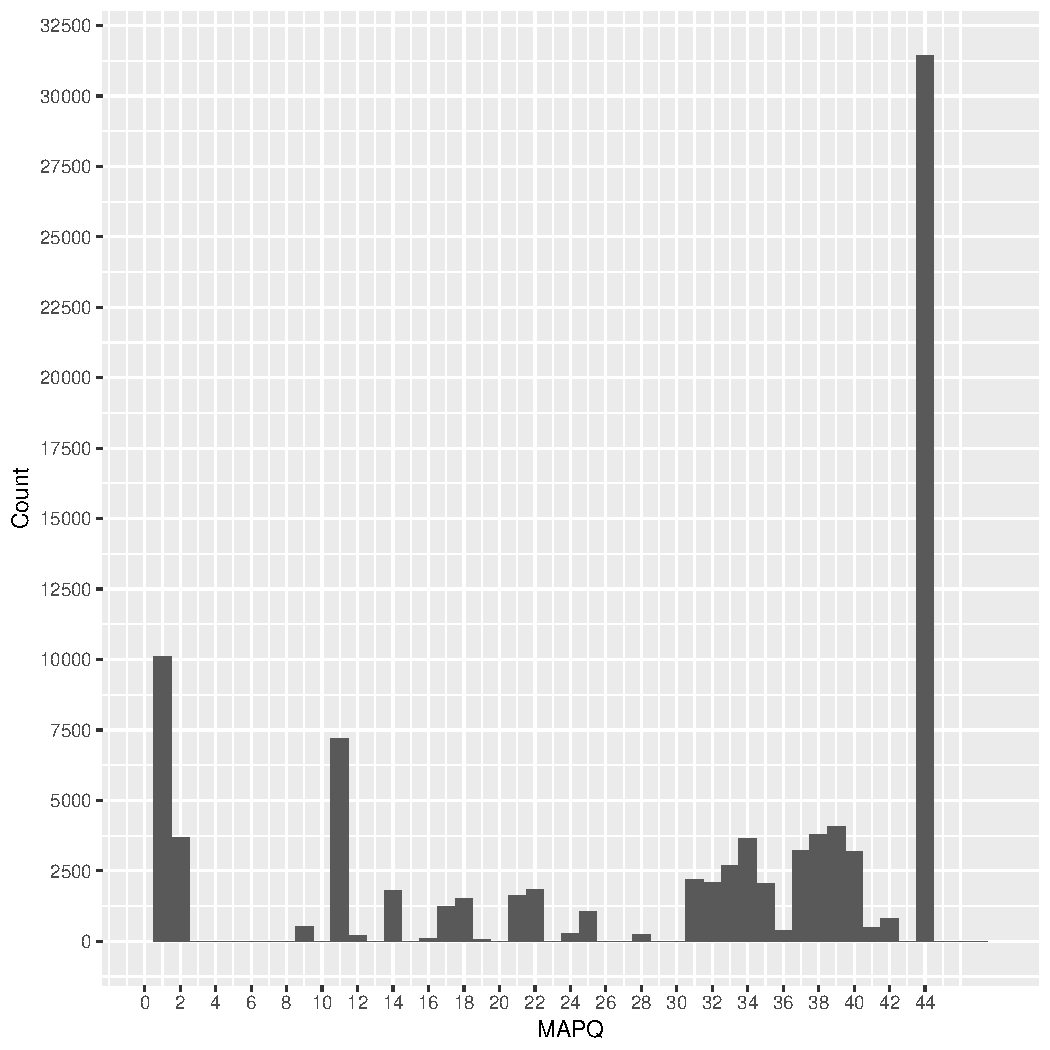
\includegraphics[width=\maxwidth]{figure/p1-1} \caption[Histogram of read's MAPQ]{Histogram of read's MAPQ}\label{fig:p1}
\end{figure}

\begin{kframe}\begin{alltt}
\hlkwd{table}\hlstd{(x} \hlopt{>} \hlnum{5}\hlstd{)}
\end{alltt}
\begin{verbatim}
## 
## FALSE  TRUE 
## 32237 77763
\end{verbatim}
\end{kframe}
\end{knitrout}
\clearpage
\subsection{Fragment Length}
\begin{knitrout}
\definecolor{shadecolor}{rgb}{0.969, 0.969, 0.969}\color{fgcolor}\begin{kframe}
\begin{alltt}
\hlstd{x} \hlkwb{<-} \hlkwd{as.data.frame}\hlstd{(purged_lens[purged_lens} \hlopt{!=} \hlnum{0}\hlstd{])}
\hlkwd{colnames}\hlstd{(x)} \hlkwb{<-} \hlstr{"len"}
\hlkwd{ggplot}\hlstd{(x,} \hlkwd{aes}\hlstd{(}\hlkwc{x} \hlstd{= len))} \hlopt{+}
        \hlkwd{geom_histogram}\hlstd{(}\hlkwc{bins} \hlstd{=} \hlnum{100}\hlstd{)} \hlopt{+}
        \hlkwd{labs}\hlstd{(}\hlkwc{x} \hlstd{=} \hlstr{"Lengths"}\hlstd{,} \hlkwc{y} \hlstd{=} \hlstr{"Count"}\hlstd{)} \hlopt{+}
        \hlkwd{scale_x_continuous}\hlstd{(}\hlkwc{breaks} \hlstd{=} \hlkwd{seq}\hlstd{(}\hlnum{75}\hlstd{,} \hlnum{550}\hlstd{,} \hlkwc{by} \hlstd{=} \hlnum{25}\hlstd{),} \hlkwc{limits} \hlstd{=} \hlkwd{c}\hlstd{(}\hlnum{75}\hlstd{,}\hlnum{550}\hlstd{))}
\end{alltt}


{\ttfamily\noindent\color{warningcolor}{\#\# Warning: Removed 38 rows containing non-finite values (stat\_bin).}}

{\ttfamily\noindent\color{warningcolor}{\#\# Warning: Removed 1 rows containing missing values (geom\_bar).}}\end{kframe}\begin{figure}[h]
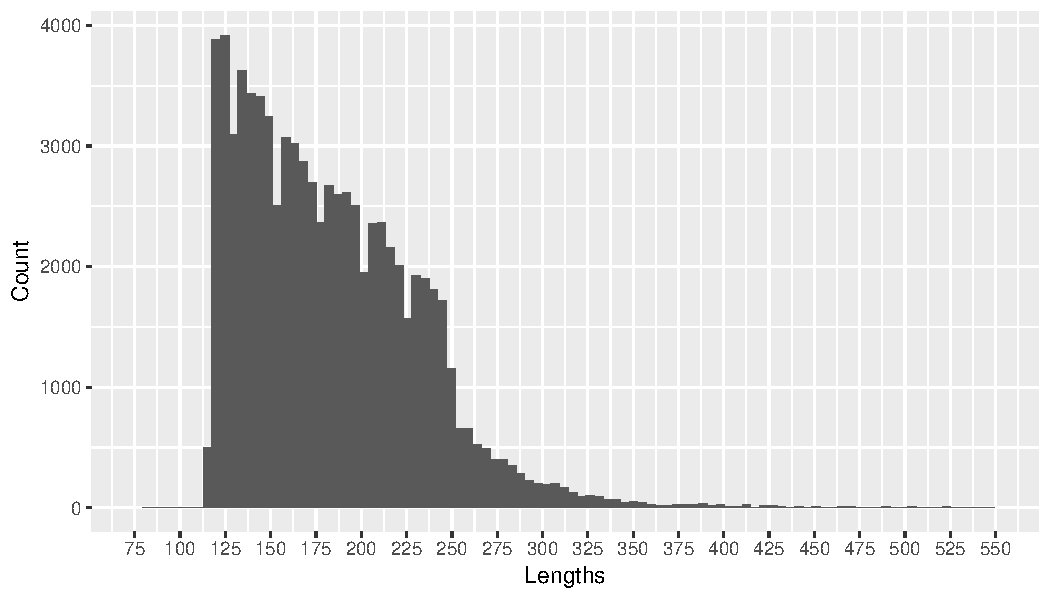
\includegraphics[width=\maxwidth]{figure/p2-1} \caption[Histogram of fragment lengths]{Histogram of fragment lengths}\label{fig:p2}
\end{figure}


\end{knitrout}

And some text after.
\end{document}
